\documentclass[arhiv]{../izpit}
\usepackage{fouriernc}
\usepackage{xcolor}
\usepackage{tikz}
\usepackage{fancyvrb}
\usetikzlibrary{calc,shapes.multipart,chains,arrows,fit,shapes}
\VerbatimFootnotes{}

\begin{document}
	
	\izpit{Programiranje I: 1. Izpit}{28.\ januar 2020}{
		Čas reševanja je 150 minut.
		Veliko uspeha!
	}
	
	%%%%%%%%%%%%%%%%%%%%%%%%%%%%%%%%%%%%%%%%%%%%%%%%%%%%%%%%%%%%%%%%%%%%%%%

	\naloga 
  
	\podnaloga Napišite funkcijo \verb|option_sum: int option -> int option -> int option|. Funkcija vrne vsoto argumentov, če oba argumenta vsebujeta število, in \verb|None| sicer.
	\begin{verbatim}
	# option_sum (Some 1) None;;
	- : int option : None
	\end{verbatim}  
  
  \podnaloga Napišite funkcijo \verb|twostep_map f l r x|, kjer imajo argumenti tipe \verb|f: ('a -> 'b * 'c)|, \verb|l: ('b -> 'd)|, \verb|r: ('c -> 'e)| in \verb|x : 'a|, rezultat funkcije pa je tipa \verb|'d * 'e|. Funkcija element \verb|x| s funkcijo \verb|f| preslika v par in na komponentah ustrezno uporabi funkciji \verb|l| in \verb|r|.
  \begin{verbatim}
  # twostep_map (fun x -> (x, x)) ((+)1) ((-)2) 3;;
  - : int * int = (4, -1)
  \end{verbatim}
  
	\podnaloga Funkcija \verb|function_repeat: ('a -> int) -> 'a list -> 'a list|, sprejme funkcijo \verb|f| in seznam \verb|list| ter vrne nov seznam, kjer se vsak element \verb|x| seznama \verb|list| ponovi \verb|f x| krat. Nepozitivno število ponovitev pomeni, da elementa ne vključimo v končni seznam. Za vse točke naj bo funkcija repno rekurzivna, kar tudi argumentirajte v komentarju.
	\begin{verbatim}
	# function_repeat (fun x -> x) [0;1;2;1;(-2)];;
	- : int list = [1;2;2;1]
	\end{verbatim}
	
	\podnaloga Definirajte funkcijo \verb|iterate: ('a -> 'a) -> ('a -> bool) -> 'a -> 'a|, ki sprejme funkcijo \verb|f|, zaustavitveni pogoj in začetno vrednost. Nato funkcijo \verb|f| zaporedoma uporablja, dokler za rezultat ne velja zaustavitveni pogoj. Funkcija naj vrne prvi rezultat, pri katerem zaustavitveni pogoj vrne \verb|true|.
	\begin{verbatim}
  # iterate (fun x -> x *. x) (fun x -> x > 12345.) 2.;; 
  - : float = 65536.
	\end{verbatim}
  
  \naloga
  
	\textit{Napreden povezan seznam} je podoben vgrajenemu seznamu v OCaml-u, le da v vozliščih namesto vrednosti hrani tabelo vrednosti (velikosti tabel niso nujno enake). Tako kot običajen povezan seznam je sestavljen iz dveh različnih gradnikov: praznega seznama in vozlišča, ki vsebuje tabelo in preostanek naprednega seznama.
	
	\podnaloga Definirajte polimorfen tip \verb|'a improved_list| ter seznam \verb|test : int improved_list|, ki predstavlja spodnji izboljšan seznam:
	% Stolen from https://tex.stackexchange.com/questions/19286/how-should-i-draw-a-singly-double-linked-list
	\[
    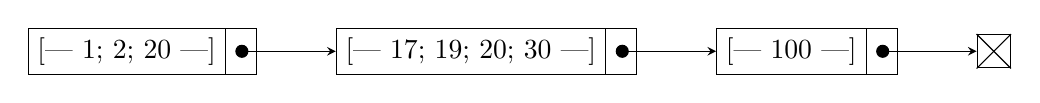
\begin{tikzpicture}[list/.style={rectangle split, rectangle split parts=2,
    	draw, rectangle split horizontal}, >=stealth, start chain]
    
    \node[list,on chain] (A) {[| 1; 2; 20 |]};
    \node[list,on chain] (B) {[| 17; 19; 20; 30 |]};
    \node[list,on chain] (C) {[| 100 |]};
    \node[on chain,draw,inner sep=6pt] (D) {};
    \draw (D.north east) -- (D.south west);
    \draw (D.north west) -- (D.south east);
    \draw[*->] let \p1 = (A.two), \p2 = (A.center) in (\x1,\y2) -- (B);
    \draw[*->] let \p1 = (B.two), \p2 = (B.center) in (\x1,\y2) -- (C);
    \draw[*->] let \p1 = (C.two), \p2 = (C.center) in (\x1,\y2) -- (D);
    \end{tikzpicture}
	\]
	
	\podnaloga Definirajte funkcijo \verb|ilist_len: 'a improved_list -> int|, ki vrne dolžino podanega seznama.
		
	\podnaloga Definirajte funkcijo \verb|get_el: int -> 'a improved_list -> 'a option|, ki vrne i-ti element če ga seznam vsebuje. Za vse točke mora biti funkcija repno rekurzivna.
	\begin{verbatim}
	# index test 5;;
	- : int option = Some 20
	\end{verbatim}
	
	\podnaloga Definirajte funkcijo \verb|is_sorted: 'a improved_list -> bool|, ki ugotovi ali je napreden seznam urejen (predpostavimo, da vsebuje elemente, ki jih lahko primerjamo z \verb|<|). Za vse točke mora biti funkcija repno rekurzivna in imeti linearno časovno zahtevnost.
	\begin{verbatim}
	# is_sorted test;;
	- : bool = false
	\end{verbatim}
	
	\podnaloga Napišite funkcijo \verb|update: 'a improved_list -> int -> 'a -> 'a improved_list|, ki vrne nov napreden seznam, kjer vrednost na indeksu (drugi argument) nadomesti s podano vrednostjo (tretji argument). Pazite, da pri tem začetni seznam ostane nespremenjen. Za vse točke mora biti funkcija repno rekurzivna, kar v komentarju tudi argumentirajte.
	\begin{verbatim}
	# index (update test 5 (-3)) 5;;
	- : int option = Some (-3)
	# index test 5;;
	- : int option = Some 20
	\end{verbatim}
	
  \naloga
  
  \podnaloga Na mizo dolžine $n$ želimo za dekoracijo postaviti $m$ posod za rože, kjer je vsaka posoda dolžine $l$. Posode za rože postavljamo eno za drugo, med dvema zaporednima posodama pa mora biti vsaj 1 enota mize prazna. Sestavite funkcijo, ki sprejme $n$, $m$ in $l$ ter vrne število vseh različnih postavitev posod za rože na mizo. Postaviti moramo vse posode, hkrati pa posod med seboj ne razlikujemo.

  Primer za vse 4 možne postavitve pri mizi dolžine 9 s tremi posodami dolžine 2:
  
  \vspace{5mm}
  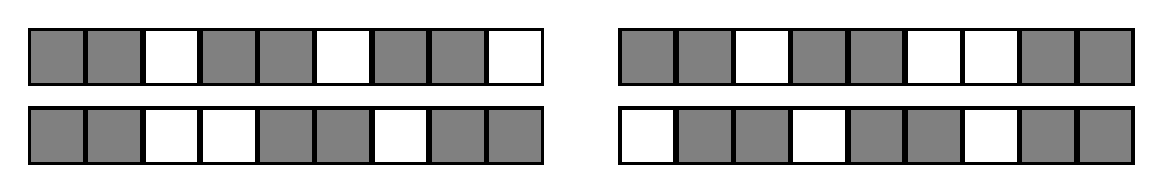
\begin{tikzpicture}
  \tikzstyle{every path}=[very thick]
  \edef\sizetape{0.7cm}
  \tikzstyle{empty}=[draw,minimum size=\sizetape]
  \tikzstyle{filled}=[draw,fill=gray,minimum size=\sizetape]
  \begin{scope}[start chain=1 going right,node distance=-0.15mm]
      \node [on chain=1,filled] {};
      \node [on chain=1,filled] {};
      \node [on chain=1,empty] {};
      \node [on chain=1,filled] {};
      \node [on chain=1,filled] {};
      \node [on chain=1,empty] {};
      \node [on chain=1,filled] {};
      \node [on chain=1,filled] {};
      \node [on chain=1,empty] {};
  \end{scope}
  \begin{scope}[shift={(7.5cm, 0cm)},start chain=2 going right,node distance=-0.15mm]
      \node [on chain=2,filled] {};
      \node [on chain=2,filled] {};
      \node [on chain=2,empty] {};
      \node [on chain=2,filled] {};
      \node [on chain=2,filled] {};
      \node [on chain=2,empty] {};
      \node [on chain=2,empty] {};
      \node [on chain=2,filled] {};
      \node [on chain=2,filled] {};
  \end{scope}
  \begin{scope}[shift={(0cm,-1cm)}, start chain=3 going right,node distance=-0.15mm]
      \node [on chain=3,filled] {};
      \node [on chain=3,filled] {};
      \node [on chain=3,empty] {};
      \node [on chain=3,empty] {};
      \node [on chain=3,filled] {};
      \node [on chain=3,filled] {};
      \node [on chain=3,empty] {};
      \node [on chain=3,filled] {};
      \node [on chain=3,filled] {};
  \end{scope}
  \begin{scope}[shift={(7.5cm,-1cm)}, start chain=4 going right,node distance=-0.15mm]
      \node [on chain=4,empty] {};
      \node [on chain=4,filled] {};
      \node [on chain=4,filled] {};
      \node [on chain=4,empty] {};
      \node [on chain=4,filled] {};
      \node [on chain=4,filled] {};
      \node [on chain=4,empty] {};
      \node [on chain=4,filled] {};
      \node [on chain=4,filled] {};
  \end{scope}
  \end{tikzpicture}
	
  \podnaloga Sedaj imamo korita različnih dolžin. Sestavite funkcijo, ki sprejme dolžino mize $n$ in seznam celih števil, ki predstavlja dolžine posod za rože, in vrne število različnih postavitev posod na mizo. Pri tem je vrstni red korit določen z vrstnim redom dolžin v podanem seznamu (med koriti iste dolžine ne razlikujemo). 
	
\end{document}